\documentclass[]{article}
\usepackage{graphicx}
\usepackage{hyperref}
\usepackage{amsmath}
\usepackage{caption}
\usepackage{subcaption}
\usepackage{float}

%opening
\title{Energy Gap in GaAs and Si}
\author{Gunther T\"urk, Jonas Lehnen}

\begin{document}

\maketitle
\begin{abstract}
In this experiment we want to measure the energy gaps for the semiconductors silicon Si and gallium arsenide GaAs. Thereby we want to see the difference between direct and indirect band transfer

\end{abstract}

\tableofcontents


\section{Theory}
\subsection{Crystallography}
There are a few different types of crystals, depending on their inner structure, they're classified into the following groups. 

The usual crystal, also called mono-crystal, is what one expects when talking about this subject. The atoms in the structure are arranged evenly as shown in >>ref<<. Every atom has its specific place and the distance between the is always the same. The classical example would be the structure of carbon in a diamond, but also semi-conductors without doping are arranged like this, due to their same amount of valence electrons. For Si and GaAs this distance is around $55\ nm$.

The polycrystalline structure is nearly a mono-crystal, but there are some spots where the connection between the atoms is broken. They are many crystals without regularity of shape and orientation. The same process can happen for a high concentration of colloids in a liquid. They can form poly-crystal like structures inside the medium they are floating in. Depending on temperature and mechanical forces, like shaking the sample, it is possible to see the crystals move in the liquid.

%%%%% 1. Grafiken ausm wiki, 2. vll ist colloids ein schlechts bsp, da es kein sollid ist

The last class are the amorphous solid bodies. In this state there is no structure in how the atoms are arranged. Most of the man-made solid bodies are considered amorphous. For example glass, polymers and thin films created by sputtering. 

\subsection{Band structure}
The band structure is derived from the Fermi-Dirac distribution. For fermions, spin=1/2 particles, there is a finite amount of how many are allowed to be in the same energy level. This results from Pauli's exclusion principle, where it's not possible to have 2 fermions with the exact same wave function. At a temperature $T=0K$ the electrons energy has to be the lowest possible. 

Considering many Coulomb potentials in a one-dimensional lattice, their energy levels overlap and shift each other apart, if they are in the same state, due to Pauli and the electromagnetic interaction between the electrons. These shifted discrete levels are still close to each other and can be merged into a band with a thickness regarding to the energy. The first band in which the electrons are no longer bound to a nucleus is called the conduction band. If an electron is this high-energetic it can be used for a current through the solid. The last band in which the electrons are still bound is called valence band. "Still bound" means that their energy is to low to leave the potential, but they are able to change the nuclei by tunneling. This is not defined as current, because the probability for tunneling into another is as low as the reversed one. The average effect is zero.

There are now three classes of solids, regarding their energy distance between valence and conduction band. This is called the energy gap. As one expects, in a metal there is no gap, electrons are free to be used a current and can change their nucleus like they want. Insulators are the extreme opposite. Their energy gap is so high, around $5eV$, that high voltage is necessary to excite them into the conduction band. This is would usually break the insulator, due to lost power as heat. 
For semi-conductors the energy gap is just less than $1eV$. This means it is possible to excite them by applying a voltage and thereby creating conductivity.

%%% doping, pn 

\subsection{Lambert Beer Law}


\section{Experiment}
\subsection{Set-up}

Via a monochromator only light of a certain wavelength can be filtered. This wavelength will later determine the energy of the light. If the lights energy is sufficient the semiconductor will be able to absorb it. In this case there will be no intensity noticeable at our photo diode. 



\subsection{Photo diode}
\subsection{Coloured filters} \label{color filters}
Now we want to see if the values the screw on the monochromator displays us is the same wavelength the coloured filters are supposed to let through. Supposing the filters information about the wavelength is more reliable than a screw with mechanical settings.

Due to the given value on the filters we checked 30 surrounding wavelengths for each filter to find each maximum. The Gaussian fits were made with the function:
\begin{equation}
f(x) = A \cdot e^{-\frac{(x-\mu)^2}{2 \sigma^2}} + b
\end{equation}

\begin{figure}[H]
\centering
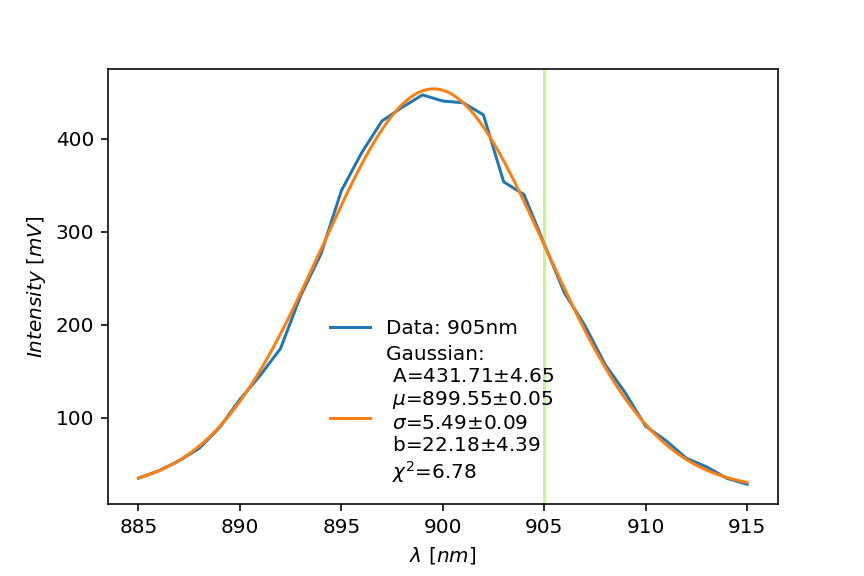
\includegraphics[width=.9\textwidth]{Plots/905nm-Filter.png}
\caption{Fit for the wavelength calibration at 905nm. Green line indicates the value given on the filters. The other filters are shown in Chapter \ref{Appendix} Appendix.}
\end{figure}

\begin{table}[H]
	\centering
	\begin{tabular}{c|c|c|c}
	Filter [nm] & 768 & 905 & 1060 \\ \hline
	Fit [nm] &  &  &  \\ \hline
	Difference [nm] &  &  & 
	\end{tabular}
	\caption{Comparison of expected and measured max intensity wavelength. The filter value is the more trustful.}
\end{table}
%%%%%%%%%%%%%%%%%%%%%%%%%%%%%%%% VALUES and how to proceed

\begin{figure}[H]
\centering
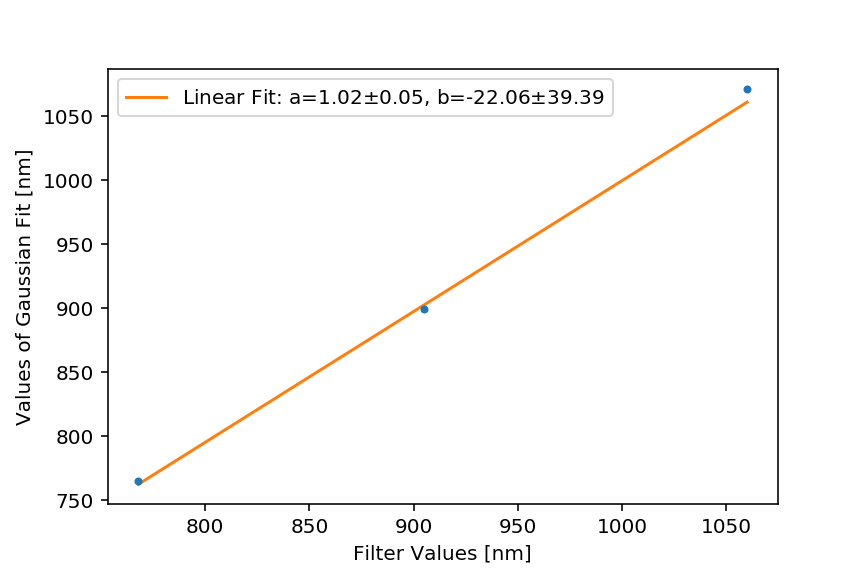
\includegraphics[width=.9\textwidth]{Plots/LambdaCorrection.png}
\caption{Correction of the monochromator values, due to the measurements with the coloured filters.}
\label{fig:LambdaCorrection}
\end{figure}

\subsection{Lamp spectrum}
In the case of changes relating to light of our lamp during the time of the experiment, we took the whole lamp spectrum before the first, in between and after the second measurement with the semiconductors in the light beam. It is possible, due to changes in temperature, that the intensities could fluctuate. This would affect the determination of the energy gap. If the plateau area is decreased, the edge could be broader and for the right sample, see <<<ref>>>>, it could be more difficult for determine a specific wavelength. But in our case nothing like this happened, as shown in figure \ref{fig:lamp spectra}.

\begin{figure}[H]
\centering
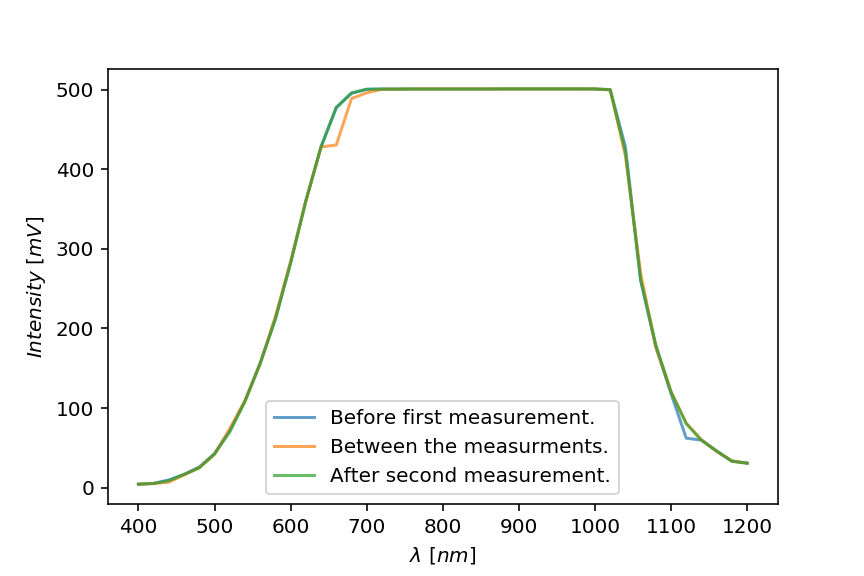
\includegraphics[width=.8\textwidth]{Plots/All-Lamp-Spectra.png}
\caption{All three measurements of the whole lamp spectrum. The measurements in the legend is related to the following measurements of the energy gaps at different temperatures. }
\label{fig:lamp spectra}
\end{figure} 

Except of some divergences, which could be caused by rapidly changing the wavelength, the spectra are nearly the same. The exact measured values are shown in Chapter \ref{Appendix} Appendix. 

This concludes in constant conditions for the energy gap measurements for silicon an gallium arsenide in the next chapter.

\subsection{Absorption edges}
\subsection{Conclusion}

\newpage
\section{Appendix} \label{Appendix}
\begin{figure}[H]
\centering
\begin{subfigure}[b]{0.9\textwidth}
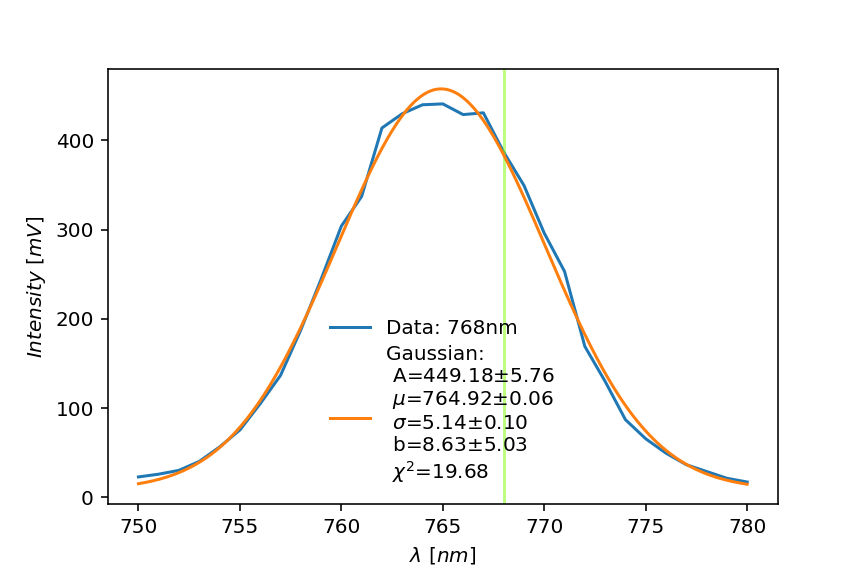
\includegraphics[width=\textwidth]{Plots/768nm-Filter.png}
\end{subfigure}
\begin{subfigure}[b]{0.9\textwidth}
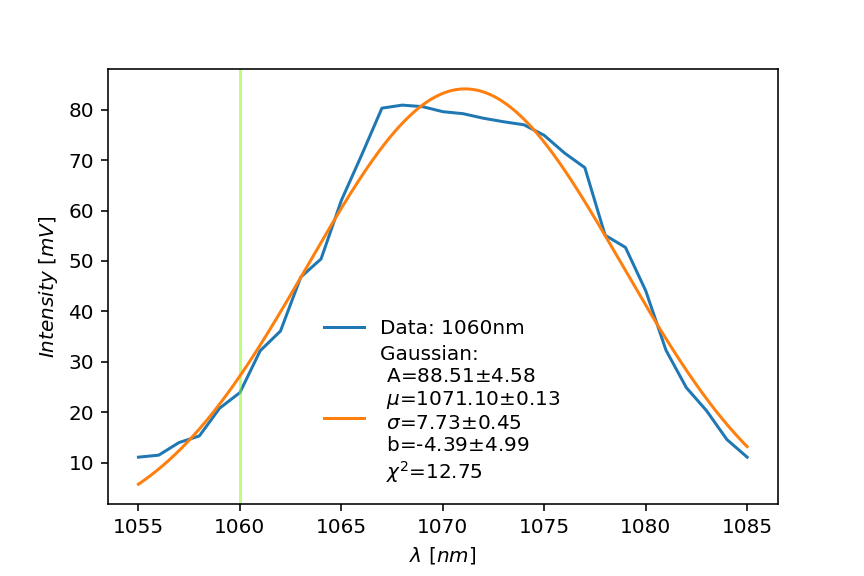
\includegraphics[width=\textwidth]{Plots/1060nm-Filter.png}
\end{subfigure}
\caption{Other filter calibrations from section \ref{color filters}. }
\end{figure}


% Tabellen der ganzen dummen Werte


\newpage
\begin{thebibliography}{}


\end{thebibliography}
\end{document}

